\chapter{Vertices and Transforms}

\begin{figure}[htb]\centering
  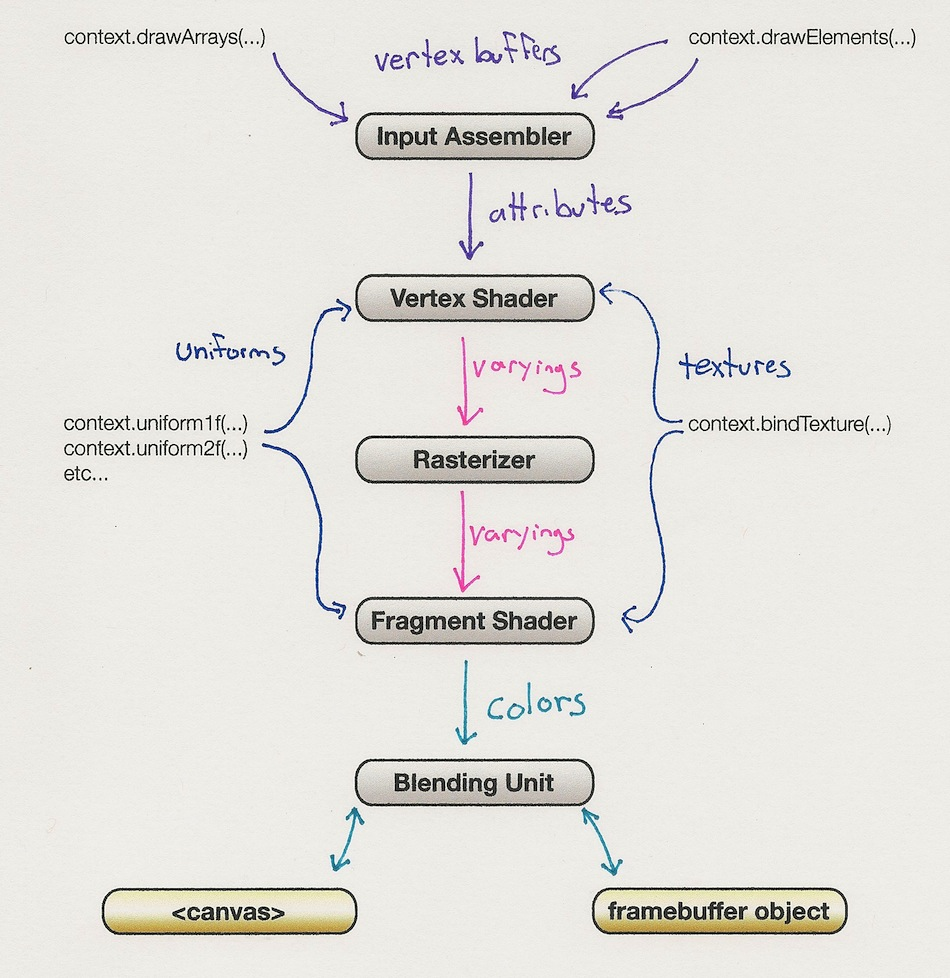
\includegraphics[width=70mm]{pipeline.jpg}
  \caption{High level view of the WebGL / OpenGL ES pipeline}
  \label{fig:AssemblyLine}
\end{figure}

\section{WebGL at 10,000 feet}
\summary{High-level overview of the WebGL rendering pipeline.}

Earlier we indicated that only two WebGL functions that can actually render 3D geometry: \code{drawArrays} and \code{drawElements}.  Both of these simply push a set of \index{vertices} \term{vertices} into the WebGL pipeline.  The vertices become rasterized into \index{fragments} \term{fragments}, or pixel values in the canvas.  Every vertex is defined by a set of \term{vertex attributes}, one of which is usually an XYZ coordinate.  Vertices come together to form \term{primitives}, which include point sprites, lines, and triangles.

Vertices initially belong to a swath of memory called a \term{vertex buffer}, and WebGL provides a rich API that allows you to specify how heterogenous attributes can be packed into a vertex buffer.  Figure~\ref{fig:AssemblyLine} depicts how vertex data flows through the pipeline, starting off in vertex buffers, eventually transforming into pixels in the canvas.

Two phases of this data flow are programmable: the vertex shader and the fragment shader.  Shaders are bundled together into \index{program object} \term{program objects}.   More precisely, a program object is the linked combination of a compiled vertex shader, a compiled fragment shader, and a set of constant inputs known as \term{uniforms}.

We'll dive deeper into shaders and vertex buffers later in this chapter; for now, see Listing~\ref{lst:Taste} for a taste of the various set-up that must be performed before actually pushing the vertices into the pipeline.

\begin{lstlisting}[
    caption={The typical state-setting that occurs before \code{drawArrays}.},
    escapechar=\%,
    label=lst:Taste,
    language=JavaScript]
// Bind a program object and set up a couple uniforms.
gl.useProgram(program);
gl.uniform1f(program, shininess, 0.5);
gl.uniform4fv(program, color, [1,1,0,1]);

// Bind a vertex buffer and set up the position attribute.
gl.bindBuffer(gl.ARRAY_BUFFER, buffer);
gl.enableVertexAttribArray(attribs.POSITION);
gl.vertexAttribPointer(attribs.POSITION, 3, gl.FLOAT, false, 0, 0);

// Finally, draw two triangles (six vertices), starting at vertex 0.
gl.drawArrays(gl.TRIANGLES, 0, 6);
\end{lstlisting}

\section{Vector Algebra with JavaScript}
\notetoself{This sections walks through giza's implementation of vector and matrix classes.  Rotation, translation, and scale are given a very brief treatment.}

\section{The Typical Life of a Vertex}
\notetoself{Describes model, view, and projection transforms.}

\section{Shading Language Basics}
\notetoself{Explains uniforms, attributes, and varyings.  Walks through trivial \texttt{main} functions for vertex and fragment shaders.}

\section{Program Objects}

\subsection{Fetching and Compiling Shader Strings}

Shaders are specified with multi-line strings that get passed to WebGL for compilation.  There are several ways to embed a multi-line string in your JavaScript code: you can end each line with a backslash, or concatenate each line with the \code{+} operator, or you can create an array of strings that can you glue together with \code{join}.

None of embedded options are ideal, so another idea is to download the entire shader from an external file, which jQuery's \code{get} method makes easy.

In this book's sample code, we've decided to use each recipe's HTML file as a container for all shader strings.  There's plenty of precendent for using \code{<script>} tags to hold things that aren't scripts.  For example, this is common when using template systems such as handlebars (\url{http://handlebarsjs.com}). 

Listing~\ref{lst:embed} shows how we embed a fragment shader in the HTML.

\begin{lstlisting}[
    language=HTML,
    caption={Embedding a shader string in HTML.},
    label=lst:embed]
<script id="simplefs" type="x-shader/x-fragment">
  precision highp float;
  varying vec3 vColor;
  void main() {
      gl_FragColor = vec4(vColor, 1.0);
  }
</script>
\end{lstlisting}

Each shader (or ``snippet'' of a shader, as we'll see later) is given a unique identifier in its enclosing script tag.  From JavaScript, this string can easily be retrieved using jQuery:

\begin{lstlisting}[language=JavaScript]
var fsText = $('#simplefs').text();
\end{lstlisting} % $

Since Giza avoids having a dependency on jQuery, it does something similar using the raw DOM element:

\begin{lstlisting}[language=JavaScript]
var fsText = document.getElementById('simplefs').innerHTML;
\end{lstlisting}

Now that we have a shader string, the next step...

\subsection{Creating Program Objects}

Recall that a \term{program object} program object is the linked combination of a compiled vertex shader, a compiled fragment shader, and a set of uniforms.

\subsection{Setting Uniforms}

\subsection{Giza's \code{compile} function}
\notetoself{Describes a useful abstraction of the WebGL program object.}

\section{Lines and Triangles}
\notetoself{Explains the various primitive types (e.g., \texttt{LINES}), \texttt{drawArrays}, and \texttt{drawElements}.}

\section{Typed Arrays, Vertex Attributes and VBOs}
\notetoself{Shows how heterogeneous data (e.g., colors and positions) can be interleaved and submitted to WebGL.}

\subsection{GIZA.BufferView}

\rrecipe{Recipe 2: Color Wheel}
\notetoself{Spinning wheel with various colors at each vertex.}
